\documentclass{standalone}

\usepackage{tikz}
\usetikzlibrary{backgrounds, positioning, shapes.symbols}
\usepackage{helvet}
\renewcommand*{\rmdefault}{\sfdefault}

\begin{document}
\begin{tikzpicture}
  [
    font=\footnotesize,
    faraday/.style={minimum size=3cm, draw, dashed},
    duplexer/.style={draw,fill=white},
  ]

  \node[label=above:porcepix] (porcepix)
    {
\includegraphics[width=1.2cm]{server}};

  \node[above right=1cm and 2cm of porcepix, label=above:asterix] (asterix)
    {
\includegraphics[width=1.2cm]{server}}
    edge (porcepix);
  \node[right=0.3cm of asterix, label=above:N310] (n310a)
    {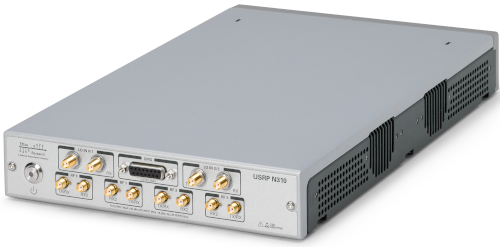
\includegraphics[width=1.5cm]{n310}} edge (asterix);
  \node[right=.2cm of n310a, duplexer] (b78o) {n78} edge (n310a);
  \node[below right=-0.1cm and 0.35cm of b78o.east] (anto1)
    {
\includegraphics[width=0.3cm]{antenna}} edge (b78o);
  \node[above right=-0.1cm and 0.35cm of b78o.east] (anto2)
    {
\includegraphics[width=0.3cm]{antenna}} edge (b78o);

  \node[right=2cm of porcepix, label=above:obelix] (obelix)
    {
\includegraphics[width=1.2cm]{server}}
    edge (porcepix);
  \node[above right=-0.5cm and 0.3cm of obelix, label=above:N310] (n310o)
    {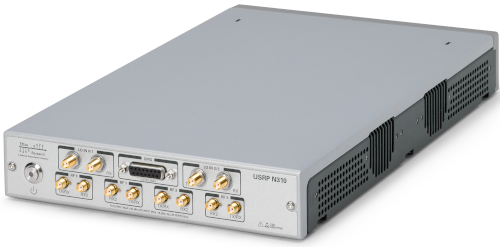
\includegraphics[width=1.5cm]{n310}} edge (obelix);
  \node[right=.2cm of n310o, duplexer] (b78o) {n40} edge (n310o);
  \node[below right=-0.1cm and 0.35cm of b78o.east] (anto1)
    {
\includegraphics[width=0.3cm]{antenna}} edge (b78o);
  \node[above right=-0.1cm and 0.35cm of b78o.east] (anto2)
    {
\includegraphics[width=0.3cm]{antenna}} edge (b78o);
  \node[below right=-0.5cm and 0.3cm of obelix, label=above:X310] (x310o)
    {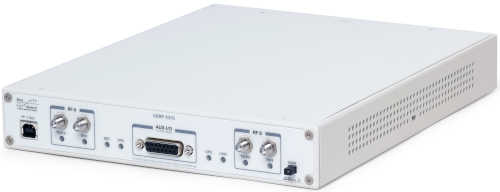
\includegraphics[width=1.5cm]{x310}} edge (obelix);
  \node[right=.2cm of x310o, duplexer] (b78o) {n78} edge (x310o);
  \node[below right=-0.1cm and 0.35cm of b78o.east] (anto1)
    {
\includegraphics[width=0.3cm]{antenna}} edge (b78o);
  \node[above right=-0.1cm and 0.35cm of b78o.east] (anto2)
    {
\includegraphics[width=0.3cm]{antenna}} edge (b78o);

  \node[above right=-1.3cm and 5.0cm of n310a.east, label=above:RM500Q-GL] (quectel)
    {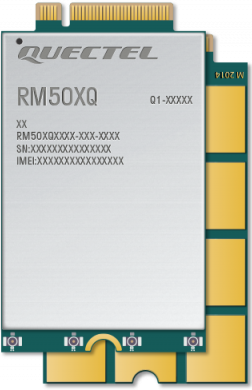
\includegraphics[height=1.2cm]{quectel}};
  \node[above left=-0.1cm and 0.8cm of quectel.west] (aq2)
    {
\includegraphics[width=0.3cm]{antenna}} edge (quectel);
  \node[above=-0.2cm of aq2] (aq1)
    {
\includegraphics[width=0.3cm]{antenna}} edge (quectel);
  \node[below=-0.2cm of aq2] (aq3)
    {
\includegraphics[width=0.3cm]{antenna}} edge (quectel);
  \node[below=-0.2cm of aq3]
    {
\includegraphics[width=0.3cm]{antenna}} edge (quectel);
  \node[right=1cm of quectel, label=above:nrmodule2] (nrmodule2)
    {
\includegraphics[width=1.2cm]{server}}
    edge (quectel);

  \node[above right=-0.3cm and 5.0cm of x310o.east, label=above:amariue] (amariue)
    {
\includegraphics[height=1.2cm]{server}};
  \node[left=0.8cm of amariue.west] (aa1)
    {
\includegraphics[width=0.3cm]{antenna}} edge (amariue);

\end{tikzpicture}
\end{document}
